% Created 2024-02-29 Thu 16:52
% Intended LaTeX compiler: lualatex
\documentclass[bigger]{beamer}
\usepackage{amsmath}
\usepackage{fontspec}
\usepackage{graphicx}
\usepackage{longtable}
\usepackage{wrapfig}
\usepackage{rotating}
\usepackage[normalem]{ulem}
\usepackage{capt-of}
\usepackage{hyperref}
\usetheme[progressbar=foot, sectionpage=none, numbering=fraction]{metropolis}
\usepackage{tikz}
\usepackage{booktabs}
\usepackage{adjustbox}
\usepackage{diagbox}
\usepackage{latexcolors}
\usetikzlibrary{automata, positioning, arrows, arrows.meta}
\usepackage{diagbox}
\usepackage{dsfont}
\usepackage{amsmath}
\usepackage{fontawesome5}
\usepackage[ruled]{algorithm2e}
\usepackage[absolute, overlay]{textpos}
\definecolor{RedBrown}{RGB}{192, 4, 4} \setbeamercolor{progress bar}{fg=RedBrown} \setbeamercolor{title separator}{fg=RedBrown}
\setbeamercolor{progress bar in head/foot}{fg=RedBrown} \setbeamercolor{progress bar in section page}{fg=RedBrown} \setbeamercolor{alerted text}{fg=RedBrown}
\pretocmd{\tableofcontents}{\thispagestyle{empty}}{}{}
\addtocounter{framenumber}{-1}
\usepackage{listings}
\usepackage{xcolor}
\definecolor{codegreen}{rgb}{0,0.6,0}
\definecolor{codegray}{rgb}{0.5,0.5,0.5}
\definecolor{codepurple}{rgb}{0.58,0,0.82}
\definecolor{backcolour}{HTML}{f0f0f0}
\lstdefinestyle{mystyle}{
backgroundcolor=\color{backcolour},
commentstyle=\color{codegreen},
keywordstyle=\color{magenta},
numberstyle=\tiny\color{codegray},
stringstyle=\color{codepurple},
basicstyle=\ttfamily,
breakatwhitespace=false,
breaklines=true,
captionpos=b,
keepspaces=true,
numbers=none,
numbersep=5pt,
showspaces=false,
showstringspaces=false,
showtabs=false,
tabsize=2
}
\lstset{style=mystyle}
\usetheme{default}
\author{Andrea Pierré}
\date{February 12\textsuperscript{th}, 2024}
\title{Lab meeting}
\subtitle{Deep dive into deep RL}
\institute{Brown University}
\titlegraphic{\hfill\includegraphics[height=1.5cm]{img/Brown Logo_2016_2 Color Process ST_1300.png}}
\setbeamercovered{transparent=10}
\setbeamertemplate{section in toc}[sections numbered]
\AtBeginSection[]{\begin{frame}[plain, noframenumbering]{Outline}    \setbeamertemplate{section in toc}[sections numbered]\setbeamertemplate{subsection in toc}[subsections numbered]\vspace{-0.8em}\tableofcontents[currentsection, currentsubsection]\end{frame}}
\AtBeginSubsection[]{\begin{frame}[plain, noframenumbering]{Outline}\setbeamertemplate{section in toc}[sections numbered]\setbeamertemplate{subsection in toc}[subsections numbered]\tableofcontents[currentsection,currentsubsection]\end{frame}}
\hypersetup{
 pdfauthor={Andrea Pierré},
 pdftitle={Lab meeting},
 pdfkeywords={},
 pdfsubject={},
 pdfcreator={Emacs 29.2 (Org mode 9.7)}, 
 pdflang={English}}
\begin{document}

\maketitle
\begin{frame}[plain]{Outline}
\tableofcontents
\end{frame}

\section{Context}
\label{sec:org85d3e4c}
\begin{frame}[label={sec:org67e8fdc}]{How do neurons in the LEC integrate sensory and spatial information?}
\begin{columns}
\begin{column}{0.45\columnwidth}
%\pause
%\scriptsize
%\footnotesize
\footnotesize
\begin{itemize}
\item \alert{Piriform Cortex} encodes olfactory information
\item \alert{Hippocampus} encodes spatial information
\item \alert{Lateral Entorhinal Cortex (LEC)} encodes both olfactory \& spatial information
\end{itemize}
\end{column}
\begin{column}{0.55\columnwidth}
\begin{center}
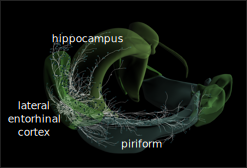
\includegraphics[width=\textwidth]{img/brain.png}
\end{center}
\end{column}
\end{columns}
\end{frame}
\begin{frame}[<+->][label={sec:org579169d}]{Why modeling?}
\begin{itemize}
\item Having a reliable model to make predictions
\item Simulation may uncover insight's from the real data
\item Derive principles from the simulation which can be checked in the experiment
\end{itemize}
\end{frame}
\begin{frame}[label={sec:orgd5f7ab7}]{The half-triangle task}
\begin{center}
\includegraphics[width=.9\linewidth]{img/RL_env-triangle-task.drawio.pdf}
\end{center}
\end{frame}
\begin{frame}[label={sec:org30fd8e0}]{Mapping states to action}
\centering
\vspace{2em}
%\fbox
\end{frame}
\section{Deep RL algorithm \& building blocs}
\label{sec:org064b4c0}
\begin{frame}[<+->][label={sec:org72678f8}]{Deep RL lessons learned}
\small
\begin{columns}
\begin{column}{0.9\columnwidth}
\begin{itemize}
\item Deep RL is different from supervised learning \(\to\) the data to optimize on is not fixed (moving target)
\item DQN tricks:
\begin{itemize}
\item \alert{Replay buffer} \(\to\) save the data experienced in a buffer and sample from it to break the temporal correlation of the data
\item \alert{Exploration warm up} with \(\epsilon\)-greedy \(\to\) experience more diverse data
\item \alert{Batching} \(\to\) update the weights of the network based on several data examples at the same time instead of only one
\item \alert{Target network} \(\to\) use 2 networks to stabilize learning (one of them is updated with a lag)
\end{itemize}
\end{itemize}
\end{column}
\begin{column}{0.1\columnwidth}
\begin{center}
\includegraphics[width=1.5\textwidth]{img/epsilon-warm-up.png}
\end{center}
\end{column}
\end{columns}
\end{frame}
\begin{frame}[label={sec:org485c29a}]{Deep RL implementation}
\SetKwComment{Comment}{/* }{ */}
\DontPrintSemicolon

\begin{center}
    \tiny
    \scalebox{0.9}{
        \begin{minipage}{\linewidth}
            \begin{algorithm}[H]
                \caption{Deep Q-Network (DQN)}\label{alg:dqn}
Initialize replay memory D to capacity N\;
Initialize action-value network Q with random weights $\theta$\;
Initialize target action-value network $\hat{Q}$ with random weights $\theta^-=\theta$\;
\For{$episode \gets 1 \dots{} M$}{
    $state \gets reset(env)$\;
    $done \gets False$\;
    \While{$done \neq True$}{
        $Q \gets forward\_pass(state)$ \Comment*[r]{4 action values vector}
        $action \gets \epsilon_{greedy}(action\_space, state, Q)$\;
        $state_{new}, reward, done \gets env.step(action, state)$\;
        Store transition (state, action, reward, next\_state, done) in D\;
        Sample random minibatch of transitions from D\;
        $Q \gets forward\_pass(state_{new})$ \Comment*[r]{4 action values vector}
        $Q_{new} \gets reward + \gamma max(\hat{Q})$ \Comment*[r]{scalar}
        $y \gets max(Q)$ \Comment*[r]{scalar}
        \eIf{$done = True$}{
            $\hat{y}_{pred} \gets reward$ \Comment*[r]{scalar}
        }{
            $\hat{y}_{pred} \gets Q_{new}$ \Comment*[r]{scalar}
        }
        $Loss \gets (y - \hat{y}_{pred})^2$\;
        Perform a gradient descent step on Loss with respect to the network parameters $\theta$\;
        Every C steps reset $\hat{Q}=Q$\;
    }
}
            \end{algorithm}
        \end{minipage}%
    }
\end{center}

\begin{textblock}{5}(1,15.5)%
\tiny
Inspired from (Mnih et al., 2015)
\end{textblock}
\end{frame}
\section{Results}
\label{sec:orgded26c5}
\begin{frame}[label={sec:orga779f7f},standout]{How deep RL feels like}
\begin{center}
\includegraphics[width=.9\linewidth]{img/blog-main-img_pen-balance-with-energel-pens.jpg}
\end{center}
\end{frame}
\begin{frame}[label={sec:org291997a}]{Networks architectures}
\centering
28 \(\to\) 54 \(\to\) 54 \(\to\) 54 \(\to\) 4
\begin{center}
\includegraphics[height=0.8\textheight]{img/nn-archi.png}
\end{center}
\end{frame}
\begin{frame}[label={sec:org9c52e50}]{Rewards \& steps}
\begin{center}
\includegraphics[height=0.29\textheight]{img/rewards-steps-1-run-working.png}
\end{center}
\begin{center}
\includegraphics[height=0.29\textheight]{img/rewards-steps-1-run-not-working.png}
\end{center}
\begin{center}
\includegraphics[height=0.29\textheight]{img/rewards-steps-avg-10-runs.png}
\end{center}
\end{frame}
\begin{frame}[label={sec:org55b9ccc}]{Loss, rewards \& steps distributions}
\begin{columns}
\begin{column}{0.3\columnwidth}
\begin{center}
\includegraphics[width=.9\linewidth]{img/loss-1-run-working.png}
\end{center}
\begin{center}
\includegraphics[width=.9\linewidth]{img/loss-1-run-not-working.png}
\end{center}
\begin{center}
\includegraphics[width=.9\linewidth]{img/loss-avg-10-runs.png}
\end{center}
\end{column}
\begin{column}{0.7\columnwidth}
\begin{center}
\includegraphics[width=.9\linewidth]{img/rewards-steps-distrib-1-run-working.png}
\end{center}
\begin{center}
\includegraphics[width=.9\linewidth]{img/rewards-steps-distrib-1-run-not-working.png}
\end{center}
\begin{center}
\includegraphics[width=.9\linewidth]{img/rewards-steps-distrib-10-runs.png}
\end{center}
\end{column}
\end{columns}
\end{frame}
\begin{frame}[label={sec:org57999e4}]{Policy learned (when it works)}
\begin{center}
\includegraphics[width=.9\linewidth]{img/policy-learned.png}
\end{center}
\end{frame}
\section{Future directions}
\label{sec:org9cd908d}
\begin{frame}[label={sec:orgdfb15e0}]{Adding memory into the task}
\begin{columns}
\begin{column}{0.5\columnwidth}
Current environment
\scriptsize
\begin{center}
\begin{tabular}{rrlr}
\hline
step & location & cue & reward\\
\hline
1 & 2 & No odor & 0\\
2 & 3 & No odor & 0\\
3 & 4 & Odor A & 0\\
4 & 3 & Odor A & 0\\
5 & 2 & Odor A & 0\\
6 & 1 & Odor A & 0\\
7 & 0 & Odor A & 10\\
\hline
\end{tabular}
\end{center}
\end{column}
\begin{column}{0.5\columnwidth}
With memorization needed
\scriptsize
\begin{center}
\begin{tabular}{rrlr}
\hline
step & location & cue & reward\\
\hline
1 & 2 & \(\emptyset\) & 0\\
2 & 3 & \(\emptyset\) & 0\\
3 & 4 & Odor A & 0\\
4 & 3 & \(\emptyset\) & 0\\
5 & 2 & \(\emptyset\) & 0\\
6 & 1 & \(\emptyset\) & 0\\
7 & 0 & \(\emptyset\) & 10\\
\hline
\end{tabular}
\end{center}
\end{column}
\end{columns}
\end{frame}
\begin{frame}[label={sec:org0a9d45b}]{RNN for memorization and sequence modeling}
\begin{center}
\includegraphics[width=0.7\textwidth]{img/RNN-transparent.png}
\end{center}
\end{frame}
\begin{frame}[label={sec:orgae42884}]{Feedback connectivity}
\begin{center}
\includegraphics[width=0.6\textwidth]{img/Network types - The Computational Brain - transparent.png}
\end{center}
\end{frame}
\begin{frame}[label={sec:orgb1819da}]{Network of networks}
\begin{center}
\includegraphics[width=.9\linewidth]{img/mRNN-transparent.png}
\end{center}

\begin{textblock}{5}(1,15)%
\tiny
(Perich and Rajan, 2020)
\end{textblock}
\end{frame}
\begin{frame}[label={sec:org5e76222},standout]{~}
Questions ?
\end{frame}
\end{document}
